\section{Lokalisering}
Når robotten skal kortlægge sine omgivelser er det nødvendigt at vide hvor den befinder sig.
Til at finde positionen har vi overvejet flere forskellige metoder.
\begin{itemize}
\item Kinect
\item Dead reckoning
\item Kamera ansigtsgenkendelse \thilemann{Er det ikke mere blob genkendelse via OpenCV der menes?}
\end{itemize}

\subsection{Kinect }
Microsofts Kinect benytter et rgb kamera samt en dybdesensor til at fortolke bevægelse som input i applikationer.
Kinect er oprindeligt lavet til XBox 360, men findes også i en version til PC, med medfølgende SDK.
En stor fordel ved at bruge Kinect er at den indeholder en dybdesensor der kan bruges til at lokalisere objekter i et rum.


\subsection{Wiimote}
En anden sensor der kan bruges er Nintendos Wiimote. 
Wiimote en optisk sensor til at lokalisere infrarødt lys fra den tilhørende sensor bar.
Ved hjælp af triangulering af det modtagne lys kan wiimoten bestemme sin position. \cite{wiimote}

\subsection{Dead reckoning}
Dead Reckoning er en teknik til at finde sin position efter ens bevægelser uden eksterne sensorer.
Robotten ved hvor den starter, og beregner sin nye position efter hvilken kommando den har udført.\cite{deadrec}

Denne teknik er ikke det bedste valg i de situationer hvor man ønsker en meget præcis lokalisering af robotten, hvilket skyldes de usikkerheder for motorer og sensorer som man ofte arbejder med.

\subsection{Valg af lokaliseringsmetode}
Der blev foretaget en indledende test af de tre foreslåede lokaliseringsmetoder for at vælge hvilken der passede bedst til dette projekt.

Dead reckoning muligheden blev hurtigt udelukket, da gruppen ville fokusere på kortlægningsopgaven og dead reckoning ville kræve en del mere arbejde end de andre lokaliseringsmetoder.

Efter sammenligning af Kinect og Wiimote blev det besluttet at fokusere på Kinect af flere årsager.
For det første havde vi adgang til en Kinect hvilket gjorde valget oplagt. 
Også det medfølgende SDK gør det let at arbejde med.
\thilemann{Her mangler lidt, f.eks. "For det andet..."?}

\subsection{OpenCV}
Til at følge et objekt på det optagne billede har vi valgt at benytte et bibliotek kaldet ``OpenCV''.
OpenCV, eller Open Source Computer Vision Library er et bibliotek der indeholder algoritmer relateret til maskinintelligens, som f.eks. genkendelse af ansigter, identificering af objekter og forfølgelse af objekter.\cite{opencv}

OpenCV bruges i dette projekt til at følge de objekter der findes ved hjælp af Kinect sensoren.

\subsection{Mapning mellem punkt på kinect og planen}
\begin{figure}
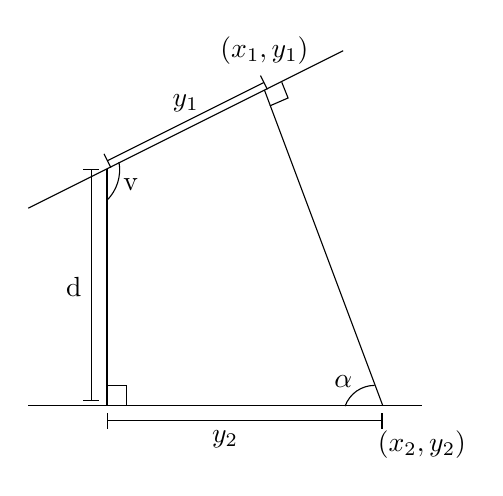
\begin{tikzpicture}

\draw (0,1) -- (5,1);
\draw (1,1) -- (1,4);
\draw (1.25,1) -- (1.25,1.25) -- (1, 1.25);
\draw (0,3.5) -- (4,5.5);
\draw (3, 5) -- (4.5,1);
\draw (3.07,4.8) -- (3.3,4.9) -- (3.22, 5.1);

\draw (1,3.6) arc [radius=0.55, start angle=-45, end angle=10];

\draw (4.4,1.25) arc [radius=0.4, start angle=-270, end angle=-200];

\node [above] at (4, 1.1) {$\alpha$};
\node [below] at (1.3,4) {v};

\draw [|-|] (0.8,1.05) -- (0.8,4);
\node [left] at (0.8,2.5) {d};

\draw [|-|] (1,0.8) -- (4.5,0.8);
\node [below] at (2.5,0.8) {$y_2$};


\draw [|-|] (1,4.1) -- (3,5.1);
\node [above] at (2,4.6) {$y_1$};

\node [above] at (3,5.2) {$(x_1,y_1)$};
\node [below] at (5,0.8) {$(x_2,y_2)$};

\end{tikzpicture}
\end{figure}

\begin{figure}
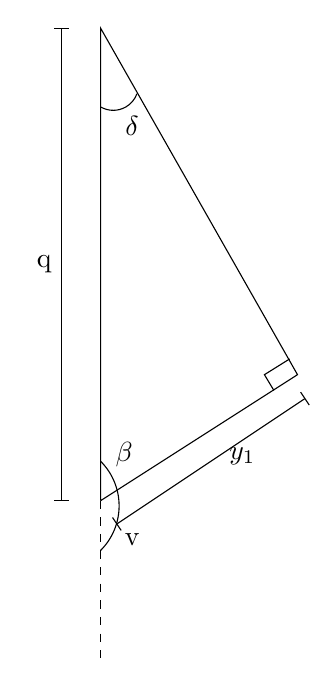
\begin{tikzpicture}[scale=2]

\draw (0,0) -- (1.25,0.8) --(0,3) -- (0,0);
\draw [dashed] (0,0) -- (0,-1);

\draw [|-|] (-0.25,0) -- (-0.25,3);
\node [left] at (-0.25, 1.5) {q};

\draw [|-|] (0.1,-0.15) -- (1.3,0.65);
\node [below] at (0.9,0.4) {$y_1$};

\draw (0,0.25) arc [radius=0.4, start angle=45, end angle=-45];
\node [above] at (0.15,0.15) {$\beta$};
\node [below] at (0.2, -0.15) {v};

\draw (0,2.5) arc [radius=0.16, start angle=-120, end angle=-20];
\node [below] at (0.2, 2.5) {$\delta$};

\draw (1.1,0.7) -- (1.04,0.8) -- (1.20,0.9);

\end{tikzpicture}
\end{figure}

\begin{itemize}
\item $\beta = 180 - v$
\item $\delta = 180 - (90+ \beta) = 90 - \beta = v-90$
\item $q = \frac{y_1}{sin(\delta)}$
\item $y_2 = tan(\delta)(q+d)$
\end{itemize}

dvs. at mapping funktionen f på formen $R \times R \times R \times R \rightarrow R \times R$ ser således ud.
$$f(x_1,y_1,v,d)=(x_1,tan(v-90)(\frac{y_1}{sin(v-90)}+d)$$
